\documentclass[12pt]{article}
\usepackage[margin=1.0in]{geometry} %page layout
\usepackage[usenames,dvipsnames]{color} %color
\definecolor{light-gray}{gray}{0.95}
\definecolor{darkgreen}{rgb}{0,0.4,0}
\usepackage{graphicx, subfigure} %figures
\usepackage{url, hyperref} %cross-referencing
\usepackage{amsmath, amssymb} %math
\usepackage{listings} %source code
\lstset{breaklines=true,
breakindent=0pt,
prebreak=\mbox{\tiny$\searrow$},
postbreak=\mbox{{\color{blue}\tiny$\rightarrow$}},
numbers=left,
commentstyle=\color{darkgreen},
numberblanklines=false,
frame=single,
captionpos=b,
backgroundcolor=\color{light-gray}}
\usepackage[3D]{movie15} %for movies (needs hyperref)
	\newenvironment{changemargin}[2]
	{
	  	\begin{list}{}
		{
			\setlength{\topsep}{0pt}%
			\setlength{\leftmargin}{#1}%
			\setlength{\rightmargin}{#2}%
			\setlength{\listparindent}{\parindent}%
			\setlength{\itemindent}{\parindent}%
			\setlength{\parsep}{\parskip}%
		}
	  	\item[]
		}
		{\end{list}
	}
\author{Salman Aslam\\Georgia Tech}
\title{Affine Warping in $\mathbb{R}^2$}
\author{Salman Aslam\\ Georgia Institute of Technology}
\date{}
\definecolor{darkgreen}{rgb}{0,0.5,0}
\newcommand{\Ntrg}{\big[N_{t=1, m=1} + \lambda \big] + \big[N_{t=1, m=2} + \lambda \big] + \ldots + \big[N_{t=1, m=M} + \lambda \big]}
\newcommand{\jointcnt}{\sum\limits_{n_{trg}=1}^{N_{trg}}I(X_t=x_t, X_{t-1}=x_{t-1})}
\newcommand{\singlecnt}{\sum\limits_{n_{trg}=1}^{N_{trg}}I(X_{t-1}=x_{t-1})}
\newcommand{\singlep}{p(X_{t-1}=x_{t-1})}
\newcommand{\singlepone}{p(X_{t-1}=1)}
\newcommand{\singleptwo}{p(X_{t-1}=2)}
\newcommand{\singlepM}{p(X_{t-1}=M)}
\newcommand{\condp}{p(X_t=x_t | X_{t-1}=x_{t-1})}
\newcommand{\jointp}{p(X_t=x_t, X_{t-1}=x_{t-1})}
\newcommand{\KmeansOuterSum}{\sum\limits_{k=1}^K}
\newcommand{\KmeansInnerSum}{\sum\limits_{{i=1 \atop x_i \in \mathcal{K}_k}}^N}
\newcommand{\KmeansSum}{\KmeansOuterSum \KmeansInnerSum}
\newcommand{\RVQInnerSum}{\sum\limits_{{i=1 \atop g_i \mapsto m_{\tau, s}}}^N}
\newcommand{\RVQOuterSum}{\sum_{s=1}^S}
\newcommand{\RVQsum}{\KmeansOuterSum \sum\limits_{{i=1 \atop g_i \in \mathcal{K}_k}}^N}
\newcommand{\KmeansInner}{{(x_i - \mu_k)}^2}
\newcommand{\RVQinner}{            {(x_i  - \hat{\mu}^{(k)})}^2}
\newcommand{\RVQinneralternate}{{(g_i - m_\tau^{(k)})}^2}
\newcommand{\RVQinneralternatealternate}{{(g_i - m_{\tau, s})}^2}
\newcommand{\KmeansError}{\KmeansSum \KmeansInner}
\newcommand{\RVQerror}     {\KmeansSum \RVQinner}
\newcommand{\RVQerroralternate}{\RVQsum \RVQinneralternate}
\newcommand{\RVQunit}{x_i -\bigg(\sum_{t=1}^Tm^{(k)}_t\bigg)}
\newcommand{\RVQequivalentCodevector}{\sum_{t=1 }^Tm^{(k)}_t}
\newcommand{\RVQequivalentCodevectorBroken}{\sum_{t=1 \atop t \neq \tau}^Tm^{(k)}_t+ m^{(k)}_\tau}
\newcommand{\RVQmultipleKmeans}{x_i -\bigg(\RVQequivalentCodevectorBroken\bigg)}
\newcommand{\RVQmultipleKmeansone}{x_i -\sum_{t=2}^Tm^{(k)}_t+ m^{(k)}_1\bigg)}
\newcommand{\RVQmultipleKmeansonealternate}{\bigg(x_i -\sum_{t=1 \atop t \neq \tau}^Tm^{(k)}_t\bigg) - m^{(k)}_\tau}
\newcommand{\RVQmultipleKmeanstwo}{x_i -\bigg(\sum_{t=1 \atop t \neq 2}^Tm^{(k)}_t+ m^{(k)}_2\bigg)}
\newcommand{\RVQmultipleKmeansT}{x_i -\bigg(\sum_{t=1}^{T-1}m^{(k)}_t+ m^{(k)}_2\bigg)}
\newcommand{\EucMatrix}
{
\left[
\begin{array}{lll}
r_{11} & r_{12} & t_x \\ 
r_{21} & r_{22} & t_y \\ 
0 & 0 & 1 \\ 
\end{array}
\right]
}	

\newcommand{\SimMatrix}
{
\left[
\begin{array}{lll}
sr_{11} & sr_{12} & t_x \\ 
sr_{21} & sr_{22} & t_y \\
0 & 0 & 1 \\ 
\end{array}
\right]
}

\newcommand{\AffMatrix}
{
\left[
\begin{array}{lll}
a &b & t_x \\ 
c & d & t_y \\
0 & 0 & 1 \\
\end{array}
\right]
}

\newcommand{\ProjMatrix}
{
\left[
\begin{array}{lll}
h_{11} & h_{12} & h_{13} \\ 
h_{21} & h_{22} & h_{23} \\ 
h_{31} & h_{32} & h_{33} \\ 
\end{array}
\right]
}

\newcommand{\RotMatrixTheta}
{
\left[
\begin{array}{rr}
\cos(\theta) & -\sin(\theta) \\ 
\sin(\theta) & \cos(\theta) \\ 
\end{array}
\right]
}

\newcommand{\RotMatrixPhi}
{
\left[
\begin{array}{rr}
\cos(\phi) & -\sin(\phi) \\ 
\sin(\phi) & \cos(\phi) \\ 
\end{array}
\right]
}

\newcommand{\RotMatrixminusPhi}
{
\left[
\begin{array}{rr}
\cos(-\phi) & -\sin(-\phi) \\ 
\sin(-\phi) & \cos(-\phi) \\ 
\end{array}
\right]
}


\newcommand{\EigenvalueMatrix}
{
\left[
\begin{array}{cc}
\lambda_1 & 0\\
0 & \lambda_2
\end{array}
\right]
}

\newcommand{\bigMatrix}
{
s \left[
\begin{array}{cc}
 (r)(a) + b &  (r)(d) - c \\
 (r)(c) - d &  (r)(b) + a
\end{array}
\right]
}


\newcommand{\bigMatrixTwo}
{
\left[
\begin{array}{cc}
(\lambda_2) p + (\lambda_1) q & (\lambda_2) s  - (\lambda_1) r \\
(\lambda_2) r  - (\lambda_1) s & (\lambda_2) q + (\lambda_1) p
\end{array}
\right]
}
\newcommand{\dr}{(\mathbf{x}_i-\boldsymbol\mu_k)^T(\mathbf{x}_i-\boldsymbol\mu_k) + \lambda({Q_{\textrm{max}}-Q_i})}

\begin{document}
\maketitle
\rule[0pt]{\textwidth}{1pt}
\tableofcontents
\rule[0pt]{\textwidth}{1pt}
%================================
\section{Introduction}
%================================
In many situations, it is necessary to track a visual target that is undergoing deformations.  Several targets of interest fall in this category, particularly non-rigid targets such as humans.  Even rigid objects can undergo severe deformation in a matter of seconds as shown in Figure~\ref{Fig:PETS2001_deformation}.  


								\begin{figure}
								\centering
								\subfigure[Frame 770.]{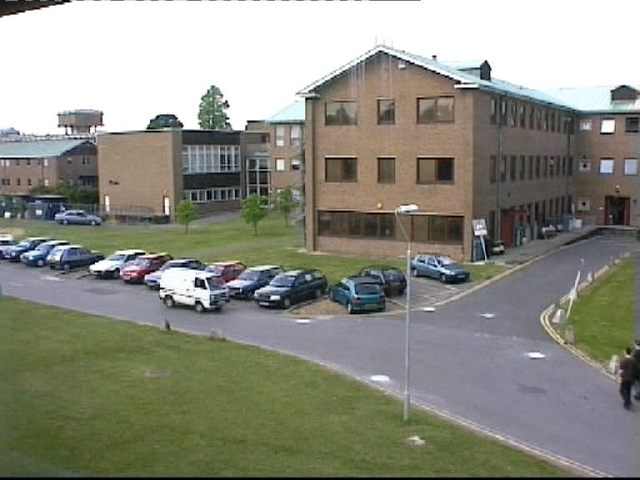
\includegraphics[width=0.45\textwidth]{figs/PETS2001_00770.jpg}}
								\subfigure[Frame 1770.]{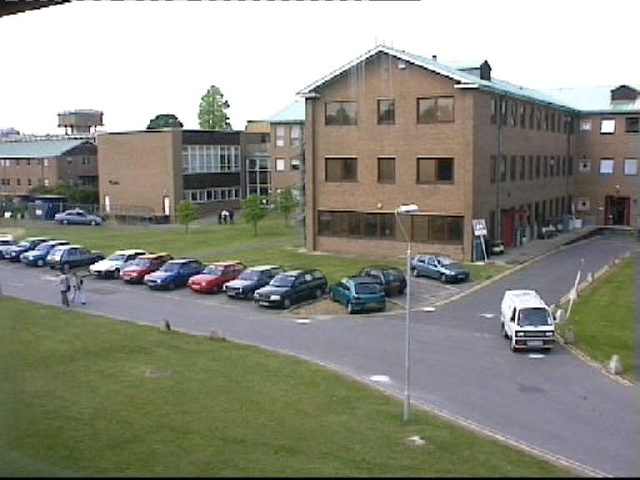
\includegraphics[width=0.45\textwidth]{figs/PETS2001_01770.jpg}}
								\caption{Over time, even rigid objects can undergo severe deformations such as the car in these images from the PETS2001 dataset.}
								\label{Fig:PETS2001_deformation}
								\end{figure}

In such cases, using a rigid rectangular bounding box to represent the target will inevitably lead to inclusion of background pixels in the matching process.  This can easily lead to tracker drift, particularly if the tracker is also trying to learn the appearance model of the target.

We now show how to use affine warping of the rectangular bounding box so that it more closely captures the outline of the target of interest.  This minimizes inclusion of background pixels in the matching process and leads to more robust tracking.

%================================
\section{Theory}
%================================
Table \ref{table:2Dtransformations} shows different kinds of 2D linear transformations.  Every transformation generalizes the transformation below it in the table.  In this report, we are interested in the 2D affine transform since it is flexible enough to account for most distortions in real images.

								\begin{table}[t]
								\centering
								\begin{tabular}{| l | c | c | p{2.5in} |}
								\hline
								Transformation & DoF & Matrix & Distortion\\ \hline 
								& & & \\ Projective & 8 & $\ProjMatrix$ & any arbitrary quadrilateral as long as no three points are collinear\\  & & & \\ \hline
								& & & \\ Affine & 6 & $\AffMatrix$ & rotation and non-isotropic scaling\\  & & & \\ \hline
								& & & \\ Similarity & 5 & $\SimMatrix$ & scaling and rigid motion\\  & & & \\ \hline
								& & & \\ Euclidean & 4 & $\EucMatrix$ & rigid motion (rotation, translation) \\  & & & \\ \hline
								\end{tabular}\
								\caption{2D transformations}
								\label{table:2Dtransformations}
								\end{table}

The affine transform\footnote{The notation adopted by some books for the affine transform is,

\begin{equation}
\begin{array}{llllllll}
X &= ax + by + e\\
Y &= cx + dy + f
\end{array}
\label{Eq:AffineDecomposition}
\end{equation}

where the input coordinate (x,y) has been transformed through 6 affine parameters, $a, b, c, d, e, f$ to the output coordinate $(X,Y)$.  Instead of $e$ and $f$, we will be using $t_x$ and $t_y$ respectively.}
 is given by,

\begin{equation}
\begin{array}{cllll}
\left[\begin{array}{l}\acute{x}\\\acute{y}\\1\end{array}\right]   &=& \AffMatrix \left[\begin{array}{l}x\\y\\1\end{array}\right]\\
\mathbf{\acute{x}} &=& \left[\begin{array}{cccc}\mathbf{A} & \mathbf{t}\\\mathbf{0}^T & 1\end{array}\right] \mathbf{x}\\
&=& \mathbf{A}\mathbf{x} + \mathbf{t}\\
&=& \mathbf{H}_A \mathbf{x}\\
\end{array}
\label{Eqn:top_level}
\end{equation}

$t_x$ and $t_y$ are translations in the $x$ and $y$ directions respectively and $\mathbf{H}_A$ is the affine transformation matrix.  The matrix $\mathbf{A}$ above can always be decomposed using the SVD decomposition as the product of orthonormal matrix $\mathbf{U}$ containing the eigenvectors of $\mathbf{A}\mathbf{A}^T$, orthonormal matrix $\mathbf{V}$ containing the eigenvectors  $\mathbf{A}^T\mathbf{A}$ and a diagonal matrix $\mathbf{S}$ containing the eigenvalues of $\mathbf{A}$~\cite{2004_BOOK_CG_Hartley}:

\begin{equation}
\begin{array}{llllllll}
\mathbf{A} &= \left[\begin{array}{lll}a & b \\ c & d\\ \end{array}\right] \\
&=\mathbf{U}{\color{darkgreen}\mathbf{S}}{\color{red}\mathbf{V}^t} \\
&={\color{blue}(\mathbf{U}\mathbf{V}^t)}{\color{red}\mathbf{V}}{\color{darkgreen}\mathbf{S}}{\color{red}\mathbf{V}^t}\\
&={\color{blue}\mathbf{R}(\theta)}{\color{red}\mathbf{R}(-\phi)}{\color{darkgreen}\mathbf{S}}{\color{red}\mathbf{R} (\phi)}\\
&={\color{blue}\RotMatrixTheta}{\color{red}\RotMatrixminusPhi}{\color{darkgreen}\EigenvalueMatrix}{\color{red}\RotMatrixPhi}\\\\
\end{array}
\label{Eq:AffineDecomposition}
\end{equation}

${\color{blue}\mathbf{U}\mathbf{V}^t}$ is an orthogonal matrix since $({\color{blue}\mathbf{U}\mathbf{V}^t})^t =({\color{blue}\mathbf{U}\mathbf{V}^t})^{-1}$.  Therefore, without loss of generality, it can be written as a rotation matrix.  Of the possible 6 DOFs (degrees of freedom) of the affine transformation, the 4 DOFs in $\mathbf{A}$, i.e., ($a, b, c$, $d$) have been replaced with $(\theta, \lambda_1, \lambda_2, \phi)$.

The affine matrix $\mathbf{A}$ can therefore be viewed as a succession of the following 4 steps:

\begin{enumerate} 
\item Rotation by angle $\phi$ 
\item This rotation is followed by a scaling of $\lambda_1$ and $\lambda_2$ in the rotated $x$ and $y$ directions
\item A rotation by angle -$\phi$ which brings the scaled object back to its original orientation
\item A rotation by angle $\theta$
\end{enumerate}

\subsection{\underline{Converting $(a, b, c, d)$ to $(\theta, \lambda_1, \lambda_2, \phi)$}}
%-------------------------------------------------
In several cases, the affine parameters are given in the form of $(a, b, c, d)$.  However, it is difficult to get a physical intuition when the parameterization is done in this form.  In such cases, converting to $(\theta, \lambda_1, \lambda_2, \phi)$ helps in getting an insight into how the object of interest is being deformed.  For this step, first compute the SVD decomposition $\mathbf{A}=\mathbf{U}{\color{darkgreen}\mathbf{S}}{\color{red}\mathbf{V}^t}$.  

The first parameter, angle $\phi$, is computed as follows,

%%%CAUTION: RECONCILE THIS WITH CODE%%%
\begin{equation}
\begin{array}{ccccll}
&{\color{red}\mathbf{R}(\phi)}&=&{\color{red}\mathbf{V}^T}\\
\Rightarrow &{\color{red}\RotMatrixPhi} &=& \left[\begin{array}{llll}v_{1,1} &v_{2,1}\\v_{1,2} & v_{2,2}\end{array}\right]\\
\end{array}
\end{equation}

Therefore,

\begin{equation}
\boxed{\phi = \tan^{-1}\frac{v_{1,2}}{v_{1,1}}}
\end{equation}

The second and third parameters, scaling factors $\lambda_1$ and $\lambda_2$, are computed as follows,

\begin{equation}
\begin{array}{ccccc}
&{\color{darkgreen}\EigenvalueMatrix} &=&{\color{darkgreen}\mathbf{S}}\\
&&=&\left[\begin{array}{cccc}s_{1,1} & 0\\0 &s_{2,2}\end{array}\right]\\
\end{array}
\end{equation}

Therefore,

\begin{equation}
\boxed{
\begin{array}{cccc}
\Rightarrow \lambda_1 &=&  s_{1,1}\\
\Rightarrow \lambda_2 &=& s_{2,2}
\end{array}}
\end{equation}

The fourth parameter, angle $\theta$, is computed as follows,  

\begin{equation}
\begin{array}{ccccc}
{\color{blue}\mathbf{R}(\theta)} &=&  {\color{blue}\mathbf{U}\mathbf{V}^T}\\
{\color{blue}\RotMatrixTheta} &= &\left[\begin{array}{llll}u_{1,1} & u_{1,2}\\u_{2,1} & u_{2,2}\end{array}\right]\left[\begin{array}{llll}v_{1,1} & v_{2,1}\\v_{1,2} & v_{2,2}\end{array}\right] \\
\end{array}
\end{equation}


Therefore,

\begin{equation}
\boxed{\theta = \tan^{-1}\frac{u_{2,1}v_{1,1} + u_{2,2}v_{1,2}}{u_{1,1}v_{1,1} + u_{1,2}v_{1,2}}}
\end{equation}

The code for this step is given in Listing~\ref{lst:UTIL_2D_affine_abcdxy_to_tllpxy}.

\subsection{\underline{Converting  $(\theta, \lambda_1, \lambda_2, \phi)$ to $(a, b, c, d)$}}
%-------------------------------------------------
In visual tracking, the initial target planar bounding region is more intuitively expressed in terms of $(\theta, \lambda_1, \lambda_2, \phi)$ than in terms of $(a, b, c, d)$.  However, the actual affine warp is more easily carried out using matrix multiplication for which we need $(a, b, c, d)$.  This can be done by multiplying out all the terms in Equation~\ref{Eq:AffineDecomposition} to get

\begin{equation}
\boxed{
\begin{array}{llll}
a &= (\lambda_2) p + (\lambda_1) q\\
b &= (\lambda_2) s  - (\lambda_1) r \\
c &= (\lambda_2) r  - (\lambda_1) s \\
d &= (\lambda_2)q + (\lambda_1) p
\end{array}}
\label{Eqn:tllpxy_to_abcdxy}
\end{equation}

								\begin{figure}
								\centering
								\fbox{
								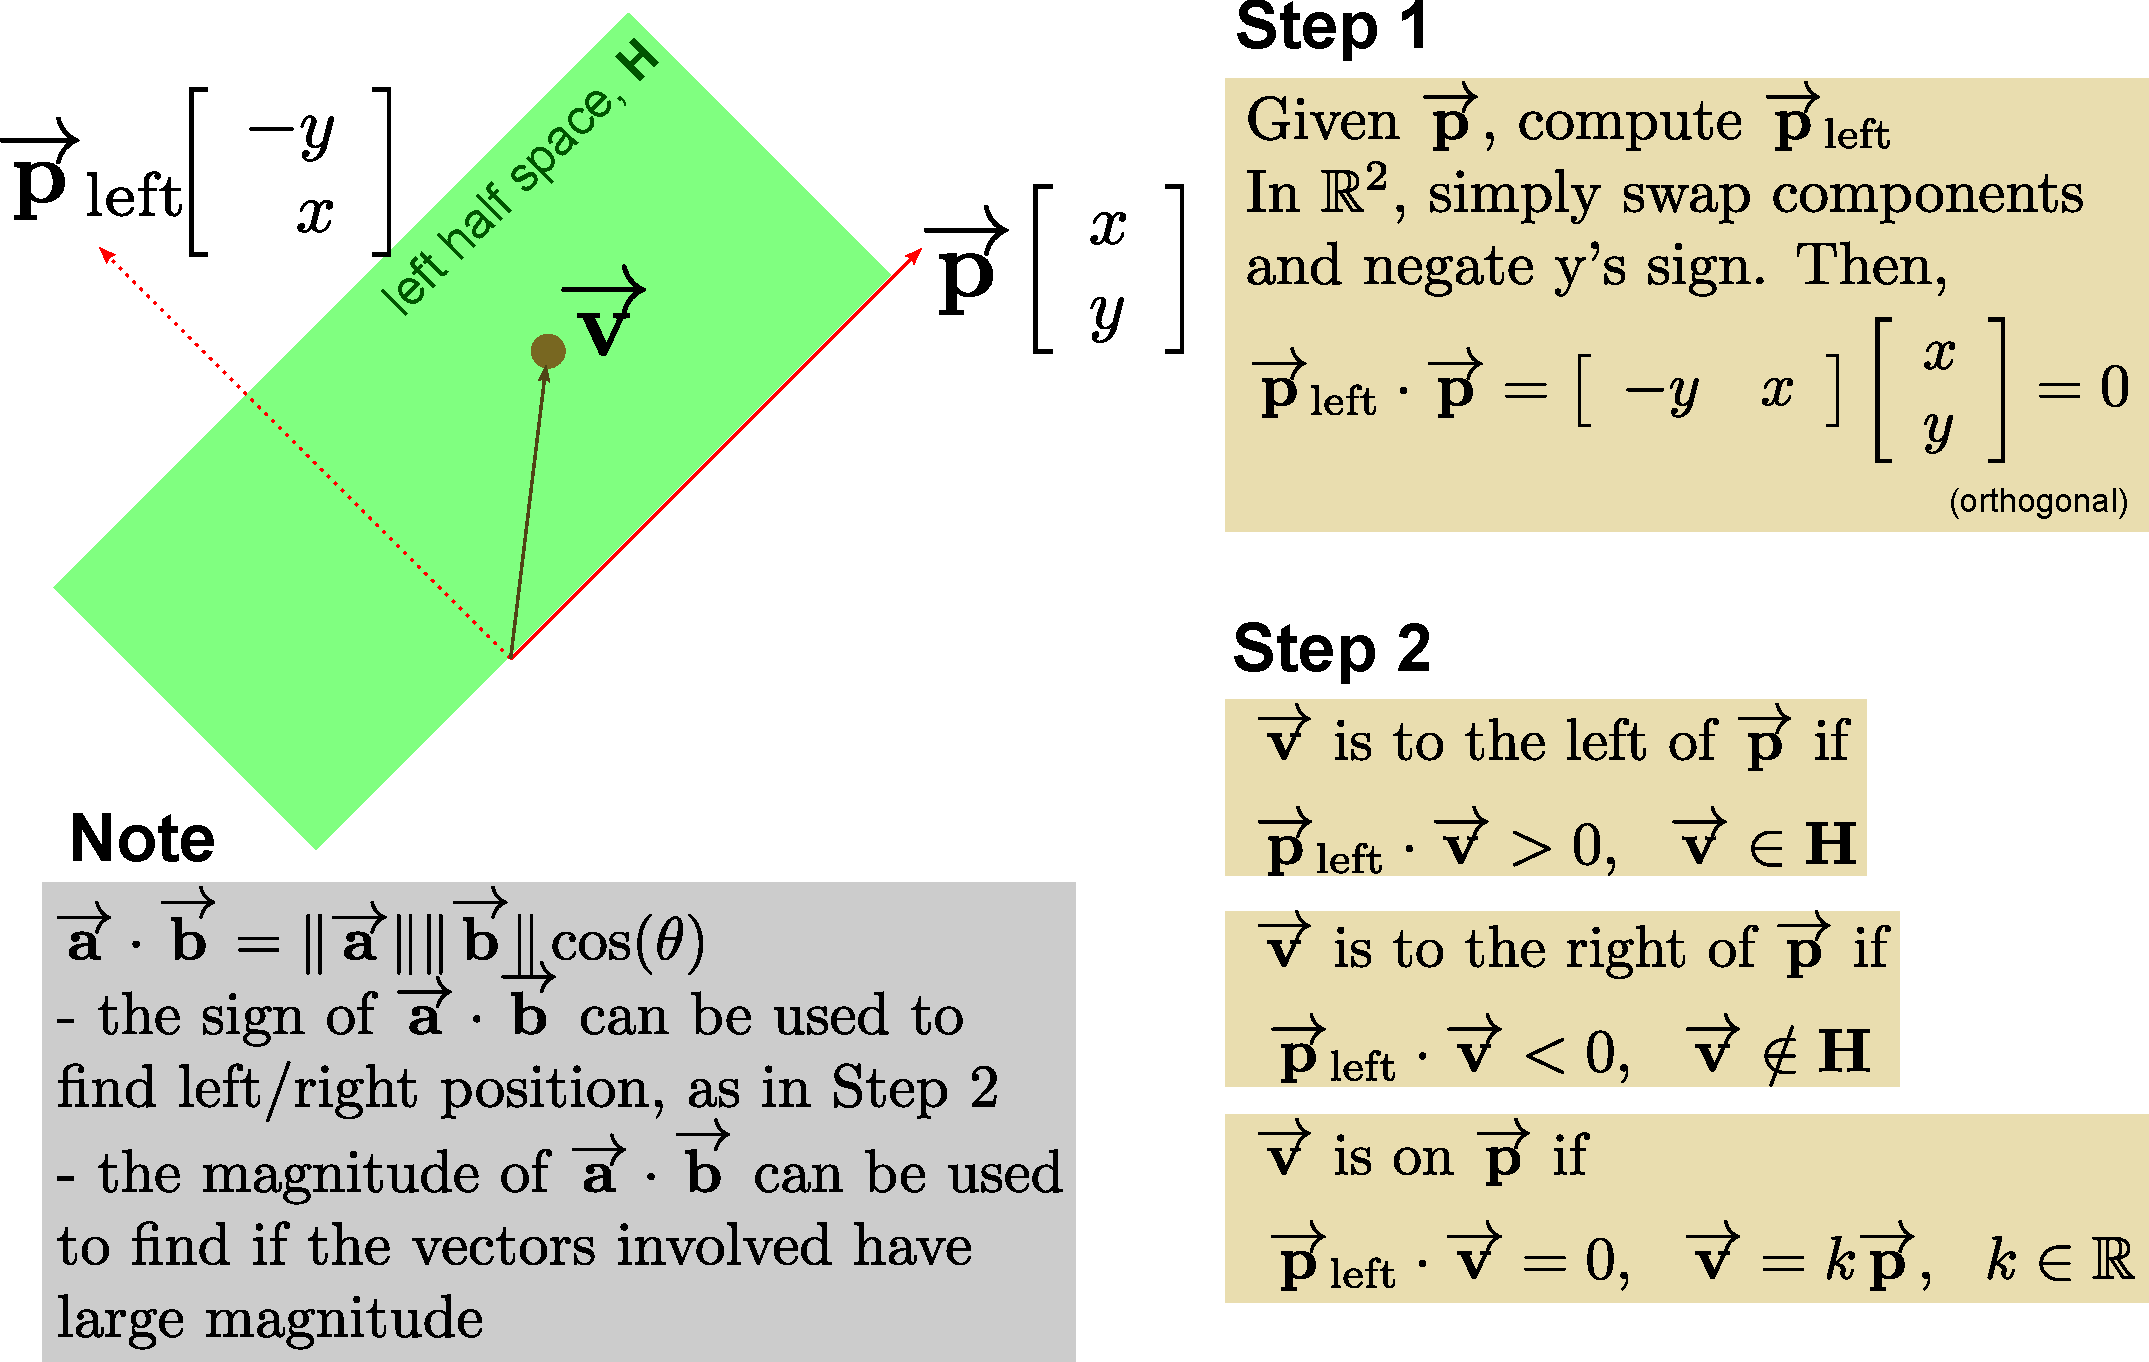
\includegraphics[width=0.75\textwidth]{figs/GRAPHICS_2D_left_turn.pdf}
								}
								\caption{Turning clockwise (left turn) in $\mathbb{R}^2$.}
								\label{fig:left_turn}
								\end{figure}


%\begin{equation}
%\begin{array}{llll}
%\mathbf{A} &= \left[\begin{array}{lll}a & b \\ c & d\\ \end{array}\right]\\
%&=\bigMatrixTwo
%\end{array}
%\end{equation}

where temporary variables $p, q, r, s$ are computed from angles $\theta$ and $\phi$ using,

\begin{equation*}
\begin{array}{llll}
\mathrm{ccc} &= \cos(\theta) \cos^2(\phi)\\
\mathrm{ccs} &= \cos(\theta) \cos(\phi) \sin(\phi)\\
\mathrm{css} &= \cos(\theta) \sin^2(\phi)\\
\mathrm{scc} &= \sin(\theta) \cos^2(\phi) \\
\mathrm{scs} &= \sin(\theta) \cos(\phi) \sin(\phi)\\
\mathrm{sss} &= \sin(\theta) \sin^2(\phi)\\
p   &=  \mathrm{css} - \mathrm{scs}\\
q   &=  \mathrm{ccc} + \mathrm{scs}\\
r   &= \mathrm{ccs} + \mathrm{sss}\\
s   &=  \mathrm{ccs} - \mathrm{scc}\\
\end{array}
\end{equation*}

The code for this step is given in Listing~\ref{lst:UTIL_2D_affine_tllpxy_to_abcdxy}.

%================================
\section{Experiments}
%================================
In our experiments, we demonstrate the following in sequence:

\begin{enumerate}
\item Manually initialize an object of interest.
\item Compute affine parameters from this manual rigid-parameter initialization.
\item Compute affine ROI (region of interest) sample points lying on object.
\item Compute actual pixel intensities on these sample points.
\end{enumerate}


								\begin{figure}
								\centering
								\subfigure[An initial zero-centered reference 33x33 grid is affinely warped to sample an object of interest.  Notice that the density of grid points is greater in the horizontal direction.]{\fbox{\includegraphics[width=0.65\textwidth]{figs/dataset_Dudek_00001_sampled2.pdf}}}
								\subfigure[Warped 33x33 output for parameters shown in the left figure.]{\includegraphics[width=0.25\textwidth]{figs/dataset_Dudek_00001_sampled3.pdf}}
								\subfigure[Different affine parameters will produce different 33x33 outputs.]{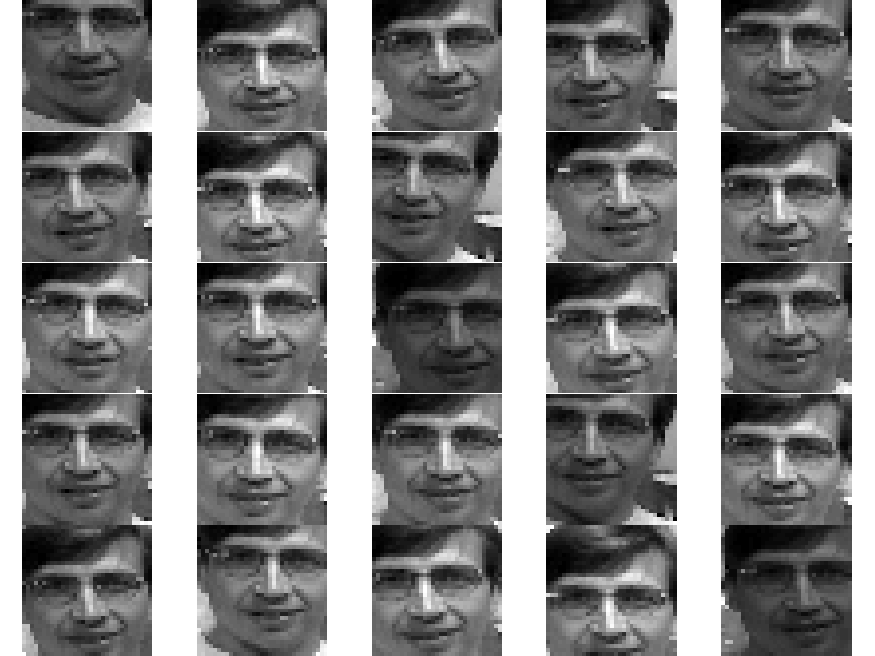
\includegraphics[width=0.65\textwidth]{figs/affineCandidates.pdf}}
								\caption{Dudek dataset, frame 1, demonstration of affine warping.  The dimensions of the object of interest, the face, are 110x130 (width x height).  The warped output is 33x33.}
								\label{Fig:affine_warping}
								\end{figure}

The source code for these steps is given in Listing~\ref{lst:demo_UTIL_2D_coordinateAffineWarping_and_IntensityInterpolation}.


\subsection{Manual initialization of object of interest}
%------------------------------------------------------------
An object of interest in an image can be manually specified by drawing a bounding box around it, and then rotating the bounding box so that it reasonably encloses the object.  This step is relatively straightforward to do in standard image processing software.  In most cases, this rigid representation, as opposed to an affine representation, will suffice to reasonably enclose the object of interest for the purposes of initialization.  This requires 5 parameters for complete specification:

\begin{enumerate}
\item $t_x$, bounding box center x coordinate
\item $t_y$, bounding box center y coordinate
\item $w$, width of bounding box
\item $h$, height of bounding box
\item $\theta$, rotation angle of bounding box in radians.  In the cartesian coordinate system, a positive $\theta$ corresponds to counter-clockwise direction.  This can be verified quickly since a $90^{\circ}$ left turn for a vector $(x,y)^T$ in $\mathbb{R}^2$ is given by $(-y,x)^T$.  This is obtained using,

\begin{equation}
\left[\begin{array}{ccc}
-y 
\\ 
x
\end{array}
\right]=
\left[
\begin{array}{rrr}
\cos(90^{\circ}) & -\sin(90^{\circ}) \\
\sin(90^{\circ}) & \cos(90^{\circ})
\end{array}
\right]
\left[\begin{array}{ccc}
x 
\\ 
y
\end{array}
\right]
\end{equation}

The term "left turn" is commonly used in computer graphics.  In  $\mathbb{R}^2$, it corresponds to a counter-clockwise rotation.  In images, where the $y$ coordinate normally decreases vertically downwards, a left turn is given by $(y,-x)^T$.  Notice that $(x,y)^T(-y,x) = (x,y)^T(y,-x) = 0$, and therefore both $ (-y,x)^T$ and $(y,-x)^T$ are orthogonal to $(x,y)^T$.  See Figure~\ref{fig:left_turn} for a graphical representation.
\end{enumerate}

As an example, consider Figure~\ref{Fig:affine_warping}.  We are interested in segmenting the face.  The initial parameters are: $t_x=188, t_y=192, w=110, h=130, \theta=-4.58^\circ$.  Note that we specify angles in radians.  $\theta$ is written here in degrees for clarity.  Moreover, notice that the bounding box is rotated in the counter-clockwise direction.  Since the y axis increases downwards, $\theta$ is negative.

\subsection{Compute affine parameters from rigid parameters}
%------------------------------------------------------------
Once we have an initial rigid representation of the object of interest, we can transform this representation into an affine representation.  Since the affine representation allows for scaling, we can scale the object and obtain its segmentation in scaled form.  For instance, in Figure~\ref{Fig:affine_warping}, the dimensions of the object of interest are 110x130.  However, for computational efficiency, we want the dimensions to be 33x33.  The affine parameters then become $\theta=-4.58^\circ, \lambda_1=110/32=3.4375, \lambda_2=130/32=4.0625, \phi=0^\circ, t_x=188, t_y=192$.  \footnote{Notice that we have divided by 32 instead of 33.  The reason is that the grid used in~\cite{2008_JNL_subspaceTRK_Ross} is 32x32 and they have accordingly used a divisor of 32.  In our case, for RVQ we require an odd dimensional grid due to the way the closed source codebook encoding software, gen.exe is setup.  Therefore, we pick a 33x33 grid.  Not changing the divisor to 33 was an oversight but this omission is expected to have minimal effect on results.}

\subsection{Compute affine coordinates (sample points) of ROI (region of interest)}
%------------------------------------------------------------
In this step, the affine parameters $(\theta, \lambda_1, \lambda_2, \phi, t_x, t_y)$ computed above are changed to $(a, b, c, d, t_x, t_y)$ using Equation~\ref{Eqn:tllpxy_to_abcdxy}.  Affine matrix $\mathbf{H}_A$ is formed using Equation~\ref{Eqn:top_level}.  A reference 33x33 grid centered on the origin is transformed using these affine coordinates to a 33x33 grid centerd on the object of interest using the affine transformation also given in Equation~\ref{Eqn:top_level}.  This can be seen in Figure~\ref{Fig:affine_warping}.

\subsection{Compute pixel intensities on these sample points}
%------------------------------------------------------------
The final step is to read off the pixel intensity values at the affinely warped grid obtained in the step above.  Most of these grid points will not have integer values.  Rounding to integer values will create artefacts.  Some form of interpolation will be required to read sub-pixel intensities.  In our experiments, we use bilinear interpolation. 


%\item \underline{Target scale and orientation changes}.  Since we choose to model the deformations in the target bounding quadrilateral with an affine transform, we can handle target scale and orientation changes.  
%\end{enumerate}
%Another aspect is that we allow for pose and scale changesthe target bounding quadrilateral to undergo affine deformation.  The state vector $\mathbf{X}$  instead of constituting the commonly used $(x,y)$ coordinates of the target now constitutes 
%================================
\section{Results}
%================================
Figure~\ref{Fig:affine_warping} shows the result of affine warping to compute grid points and bilinear interpolation to compute pixel intensities.  We see that the affine region of interest accurately samples the object of interest and minimizes inclusion of background pixels.  Also, bilinear interpolation produces an accurate representation of the target of interest.  Also shown are other outputs for a set of random perturbations of our affine parameters.  These outputs can for instance be candidate samples for a particle filter.

%================================
\section{Conclusions}
%================================
Affine warping is an effective way of downsampling an object of interest as well as allowing a region of interest to be defined that minimizes inclusion of background pixels.


%-----------------------------------------------------------------
\newpage
\appendix
\section{Source code}
\label{Sec:sourceCode}
%-----------------------------------------------------------------
\scriptsize

\lstinputlisting[language=Matlab, caption={demo\_UTIL\_2D\_coordinateAffineWarping\_and\_IntensityInterpolation.m}, 		label=lst:demo_UTIL_2D_coordinateAffineWarping_and_IntensityInterpolation]			{demo_UTIL_2D_coordinateAffineWarping_and_IntensityInterpolation.m}
\lstinputlisting[language=Matlab, caption={UTIL\_2D\_coordinateAffineWarping\_and\_IntensityInterpolation.m}, 		label=lst:UTIL_2D_coordinateAffineWarping_and_IntensityInterpolation]			{UTIL_2D_coordinateAffineWarping_and_IntensityInterpolation.m}
\lstinputlisting[language=Matlab, caption={UTIL\_2D\_affine\_apply\_transform.m}, 		label=lst:UTIL_2D_affine_apply_transform]		{UTIL_2D_affine_apply_transform.m}
\lstinputlisting[language=Matlab, caption={UTIL\_2D\_affine\_A\_2x3\_from\_abcdxy.m}, 	label=lst:UTIL_2D_affine_A_2x3_from_abcdxy]	{UTIL_2D_affine_A_2x3_from_abcdxy.m}
\lstinputlisting[language=Matlab, caption={UTIL\_2D\_affine\_abcdtxty\_to\_tllpxy.m.}, 	label=lst:UTIL_2D_affine_abcdxy_to_tllpxy]		{UTIL_2D_affine_abcdxy_to_tllpxy.m}
\lstinputlisting[language=Matlab, caption={UTIL\_2D\_affine\_tllpxy\_to\_abcdxy.m.}, 		label=lst:UTIL_2D_affine_tllpxy_to_abcdxy]		{UTIL_2D_affine_tllpxy_to_abcdxy.m}
%\lstinputlisting[language=Matlab, caption={affparaminv.m.}, 								label=lst:affparaminv]								%{affparaminv.m}
\lstinputlisting[language=Matlab, caption={UTIL\_2D\_make\_rotation\_matrix.m}, 			label=lst:UTIL_2D_make_rotation_matrix]			{UTIL_2D_make_rotation_matrix.m}

\normalsize
\bibliographystyle{ieee}
\bibliography{MyCitations}
\end{document}